%% The following is a directive for TeXShop to indicate the main file
%%!TEX root = diss.tex

\chapter{Introduction}
\label{ch:Introduction}

%%%%%%%%%%%%%%%%%%%%%%%%%%%%%%%%%%%%%%%%%%%%%%%%%%%%%%%%%%%%%%%%%%%%%%
\section{Motivation}
\label{sec:Motivation}

Since the neutrino was first postulated by Wolfgang Pauli in 1930 \cite{neutrinoHistory}, investigation into their properties has presented a significant challenge for physics researchers, with a great impact on our understanding of the universe.
Because neutrinos do not react via the electromagnetic force, they may only be detected via the weak force.

There are three flavors of neutrinos: the electron neutrino $\nu_e$, the muon neutrino $\nu_\mu$, and the tau neutrino $\nu_\tau$.
In 1998, the Super-Kamiokande detector in Japan observed clear evidence of neutrino oscillation: as neutrinos of one flavor travels over a large distance, it has some probability of later being observed as a neutrino of another generation.
This implied that neutrinos have a nonzero mass, a result not predicted by the Standard Model.
The theorized explanation for neutrino oscillation is that each neutrino flavor actually exists as some superposition of 3 different mass states - as a neutrino travels over large distances, the differences in phases of the mass states results in a shifting probability of detecting each neutrino flavor.
The relationship between mass and flavor states is governed by the following relation:

\[
\begin{pmatrix}
\nu_e \\ \nu_\mu \\ \nu_\tau
\end{pmatrix}
=
U \begin{pmatrix}
\nu_1 \\ \nu_2 \\ \nu_3
\end{pmatrix}
\]

Here, U is a $3 \times 3$ unitary matrix, known as the PMNS Matrix.
The matrix can be characterized by 4 parameters: $\theta_{12}, \theta_{23}, \theta_{13}$, which are the "mixing angles", and $\delta_{CP}$, known as the CP-violating phase \cite{pdg2018}. 

There are many open-ended questions regarding neutrinos.
The parameters of the PMNS Matrix are poorly constrained.
% TODO: SEPARATE OUT SENTENCES FOR EACH LINE AFTER THIS
The neutrino masses are currently unknown, nor is it known why their masses are so small, nor are the mass orderings of the three states known.
It is unknown whether neutrinos are their own anti-particles (i.e. whether the neutrino is a Majorana fermion), or if the antineutrino is a distinct particle (i.e. a Dirac fermion). It is uncertain whether the $\delta_{CP}$ is consistent with zero: If it is nonzero, then that may explain the asymmetry between the amount of matter and antimatter in the universe \cite{neutrinoCP}.

The Super-Kamiokande experiment that first observed neutrino oscillations did so by observing atmospheric neutrinos: upon collision with atoms in the earth's atmosphere, energetic cosmic rays produce a shower of secondary particles such as pions and muons - some of these particles then produce neutrinos when they decay. Another source of neutrinos ideal for oscillation experiments are through particle accelerators. When an sufficiently energetic proton beam hits a target, the collision produces secondary particles: charged pions and kaons. The charged pions will decay in flight as follows:
% \text{and} \
$$ \pi^+ \rightarrow \mu^+ + \nu_\mu \quad \quad \mu^+ \rightarrow \bar{\nu}_e + \nu_\mu$$

The charged kaons have several decay modes, but the most common are:
% \text{and} 

$$ K^+ \rightarrow \mu^+ + \nu_\mu \quad \quad K^+ \rightarrow \pi^+ + \pi^0$$

with corresponding charge-conjugate decays for the $\pi^-$ and $K^-$. Due to the high momentum of the secondary particles, these decays then produce a directed beam of neutrinos. This allows them to travel the great distances to neutrino detectors necessary to observe oscillation.

The next generation of neutrino experiments include DUNE and the Hyper-Kamiokande experiment. 

NA61/SHINE successful for T2K, had some inconsistencies, and did not hit a full range of beam momenta

 \section{The EMPHATIC Experiment}

In order to constrain hadron production flux uncertainties, work is in progress for the EMPHATIC (Emulsion-based Measurement of the Production of Hadrons At a Test-beam In Chicagoland) experiment. EMPHATIC is a tabletop experiment designed to precisely measure hadron interactions resulting from a proton beam impinging on various targets. EMPHATIC is located at the Fermilab Test Beam Facility, and the proposed experimental setup is shown in Figure \ref{fig:EMPHATIC}.

\begin{figure}[] 
\centering
\resizebox{0.8\textwidth}{!}{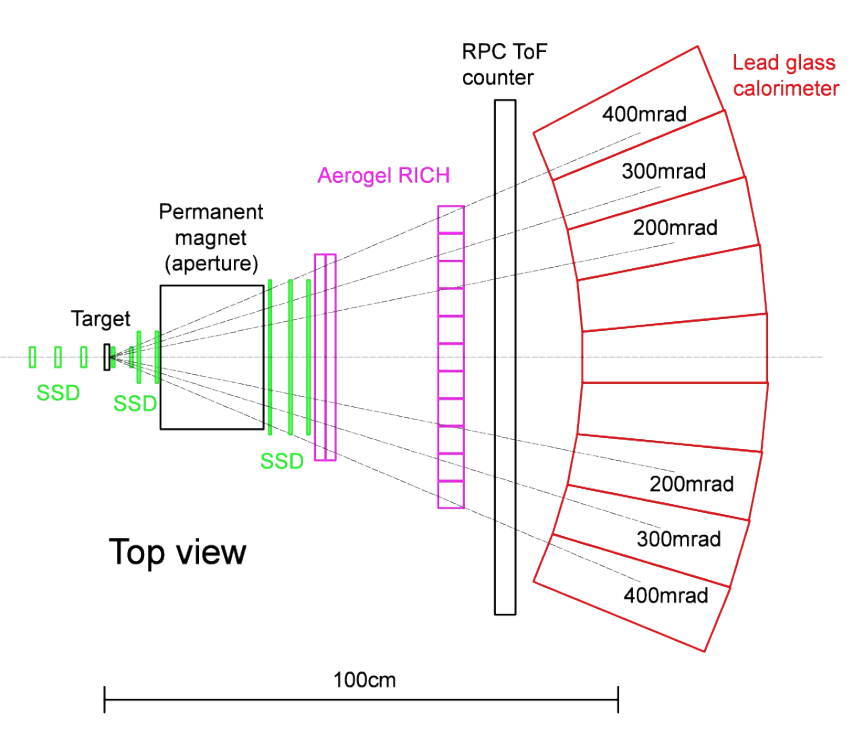
\includegraphics{./figs/EMPHATIC.png}}
\caption{Top view of the proposed EMPHATIC setup, obtained with permission from the EMPHATIC group. The different detectors in the setup are shown in different colours. The Aerogel RICH detector, RPC ToF counter, and Permanent magnet are all currently being developed.}

\label{fig:EMPHATIC}       % Give a unique label to the figure. 
\end{figure}

To obtain measurements for accelerator-based neutrino experiments, EMPHATIC will measure targets of graphite, aluminum, and iron. These targets correspond to the composition of the proposed targets, magnetic horns, and beamline components typically found in accelerator-based neutrino experiments. EMPHATIC will also measure targets composed of boron, boron nitride, and boron trioxide. Because the atmosphere is primarily composed of nitrogen and oxygen, measuring the latter two targets and removing the effects of the former will lead to estimation of hadron production in the interaction of cosmic rays in the atmosphere. 

In order to measure the production of hadrons, EMPHATIC includes four different kinds of detectors. A set of silicon strip detectors (SSDs) register the position of each particle as they pass through. A permanent magnet downstream of the target causes the trajectory of particles to curve due to the Lorentz force: the radius of the curvature depends on the momentum of the particle, so using SSDs downstream of the magnet allows for the measurement of particle momenta and trajectory. The particles then pass through an Aerogel Ring Imaging Cherenkov (ARICH) detector. As explained in Section \ref{sec:ARICH}, this detector can be used to determine a charged particle's velocity if its trajectory is known. If the velocity $\bf{v}$ and momentum $\bf{p}$ of a particle are known, then the its mass may be determined by the relativistic equation:

\begin{equation}
    \label{eq:relMass}
    m = \frac{\bf{p}}{\bf{v}}\sqrt{1-\frac{v^2}{c^2}}
\end{equation}
where $c$ is the speed of light in a vacuum. This allows for the identification of each particle.

After passing through the ARICH, particles will pass through a resistive plate chamber time-of-flight (RPC ToF) detector. This detector simply measures the time taken for a particle to travel some short distance, giving another measure of velocity. The RPC ToF has a lower resolution at the higher particle velocities measured by the ARICH detector, so these two detectors complement each other to provide a full measurement of velocities across a broad range.

After passing through the the RPC ToF, the particles strike a lead glass calorimeter, which measures the final particle energy. The lead glass calorimeter is useful for detecting any electrons or neutrons.

Currently, development is underway on the simulation and design of the ARICH detector. The ARICH detector should be able to accurately distinguish between the charged pions, charged kaons, protons, and electrons over a broad spectrum of momenta. In order to meet these goals, it is crucial that simulations be done to characterize the detector's performance and optimize the design. There are many elements of randomness in the propagation of particles through the detector, which necessitates the use of Monte Carlo simulations. 




\endinput

Any text after an \endinput is ignored.
You could put scraps here or things in progress.
